\chapter{Numerical model} \label{chap:discretization} %discretized equations?
In this chapter we describe the methods that are used to discretize the model. 
For the spatial discretization we use the finite volumes method, which allows 
to solve efficiently flow problems guaranteeing the mass conservation. See 
\cite{fv:leveque} for a broad description.
In the free-flow region we discretize the equations using the staggered grid 
concept, while in the porous-medium we employ a cell-centred approach with a 
Two Point Flux Approximation (TPFA).

For the temporal discretization we use implicit finite differences methods, 
like Backward Euler (BE) and the Backward Differencing Formula 2 (BDF2).
%
\section{Staggered grid concept}
The staggered grid concept is characterized by the distinction between the 
degrees of freedom related to scalar primary variables and those related to 
vectorial primary variables. In saddle point problems, like the incompressible 
Navier-Stokes or RANS equations, if we locate all the primary variables, i.e. 
pressure, velocity and possibly the turbulent kinetic energy and its 
dissipation rate, at the same positions in the grid, spurious modes in the 
solution may arise, leading to wrong results. A possible fix to this issue 
is thus to store the variables in a \emph{staggered} fashion, putting 
the degrees of freedom related to scalar variables at the centre of the cells 
and those related to vectorial variables on the faces, aligned to the faces 
normal direction. Therefore we obtain different control volumes, as we can see 
in Figure~\ref{fig:staggrid} for the case of the 
Navier-Stokes equations in a two-dimensional domain.
\begin{figure}[t]
	\centering
%	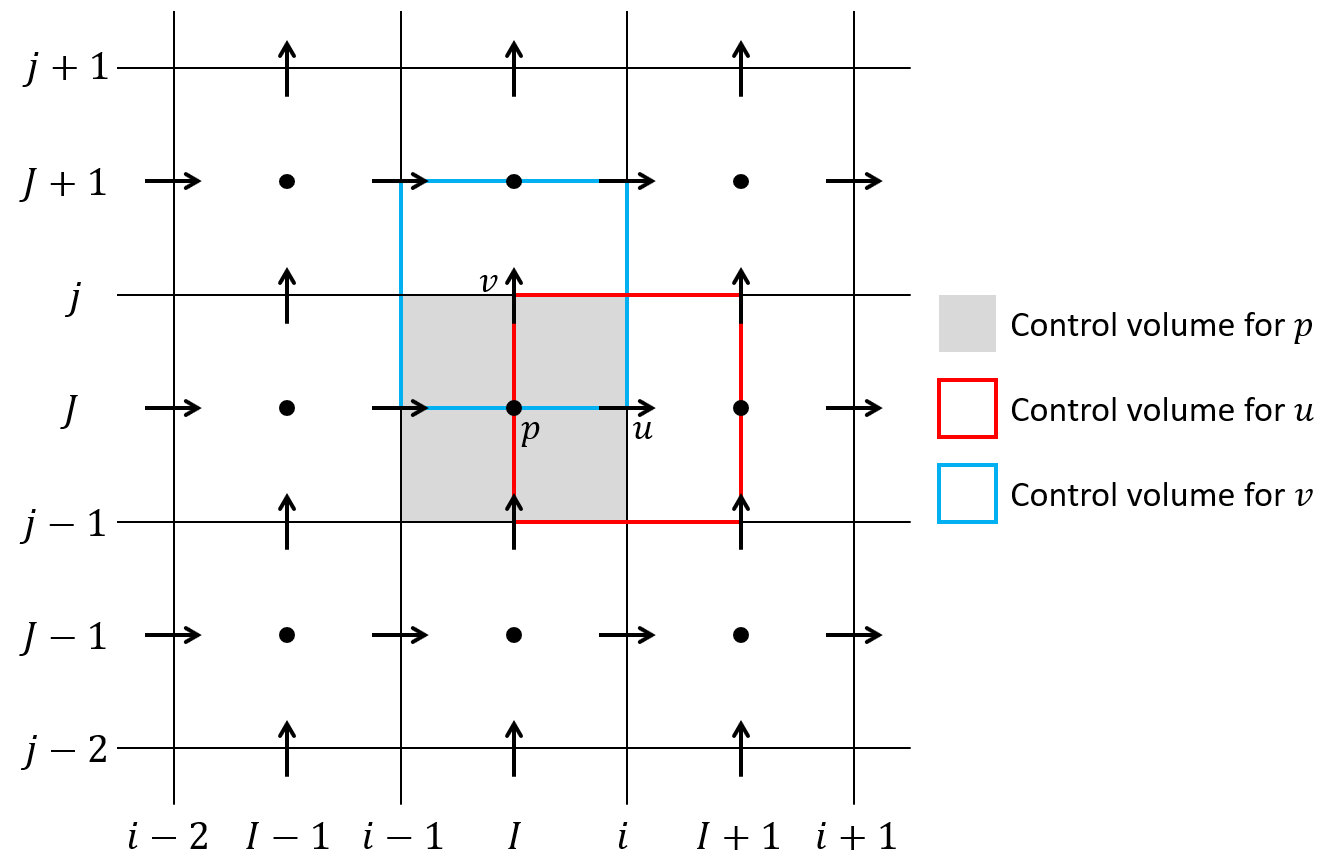
\includegraphics[width=\textwidth]{staggered_grid_mia_ij.png}
	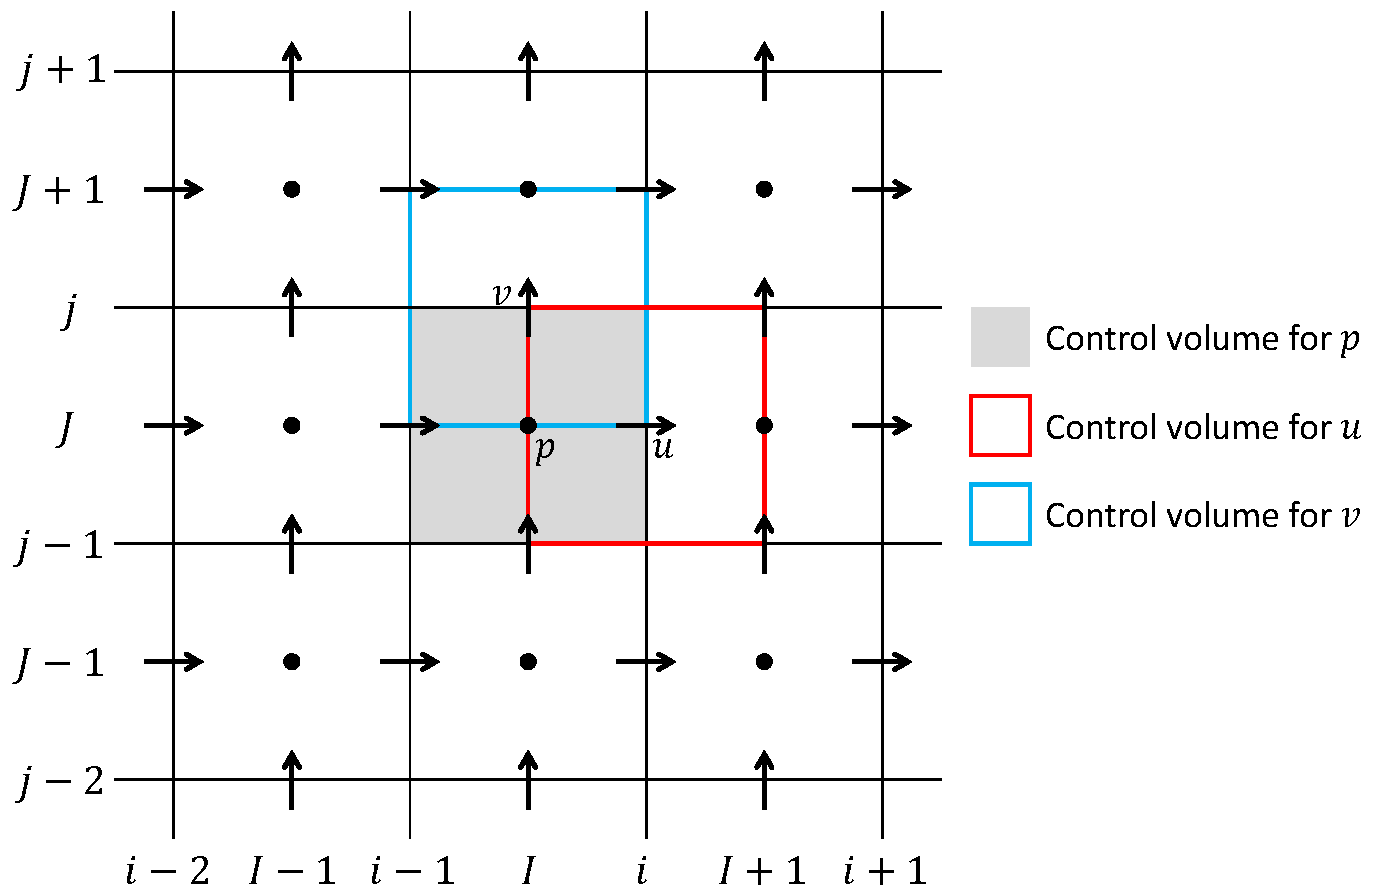
\includegraphics[width=\textwidth]{staggered_grid_mia.pdf}
	\caption[Staggered grid control volumes]{An example of a staggered grid 
	with the pressure degrees of freedom (dofs) stored at the centres of the 
	cells and the velocity dofs stored on the faces. The different control 
	volumes are highlighted. The indices in capital letters 
	$\dots,I-1,I,I+1,\dots$ 
	and $\dots,J-1,J,J+1,\dots$ refer to cells, thus to the position of 
	cell-centred variables, while the indices in lower case letters 
	$\dots,i-1,i,i+1,\dots$ and $\dots,j-1,j,j+1,\dots$ refer to faces, thus to 
	the 
	position of staggered variables.}
	\label{fig:staggrid}
\end{figure}

This approach is known also as Marker and Cell (MAC), as it was called in its 
first appearance in a paper by \textcite{stagg:orig}, within a finite 
differences framework. A more recent description can be found in 
\cite{main:vermal}.

Another advantage of this discretization method is that on the boundary we have 
the degrees of freedom of the normal component of the velocity, so it is easier 
to impose boundary and interface conditions.

For the sake of simplicity we consider now a bi-dimensional domain and 
$\mathbf{v} = [u, v]^{\mathrm{T}}$.
%
\subsection{Cell-centred equations}
\subsubsection{Continuity equation}
The continuity equation \eqref{eq:ransmass} is discretized using control 
volumes that coincide with the cells of the grid, thus it is treated is a 
cell-centred way. Since we are dealing with incompressible fluids, it does not 
involve the density and this makes its approximation easier.
%We will see in section ... how to deal with non constant desities
We integrate over the ``grey'' control 
volume $V_p = [x_{i-1},x_i] \times [y_{j-1},y_j]$, according to 
Figure~\ref{fig:staggrid}, 
and we apply the Gauss's divergence theorem:
\begin{equation}
\int_{V_p} \nabla \cdot \mathbf{v} \; dV = \int_{\partial V_p} \mathbf{v} \cdot 
\mathbf{n} \; dA = 0.
\end{equation}
The integral over the boundary $\partial V_p$ can be split over the four faces, 
that we identify with $e_p$ (east), $n_p$ (north), $w_p$ (west), $s_p$ (south):
\begin{equation}
\int_{\partial V_p} \mathbf{v} \cdot \mathbf{n} \; dA = \int_{e_p} u \; dA
+ \int_{n_p} v \; dA - \int_{w_p} u \; dA - \int_{s_p} v \; dA.
\end{equation}
At this point we discretize the equation approximating the values of the 
velocity with the values at the centre of the faces, for example:
\begin{equation}
\int_{e_p} u \; dA \approx u_{i,J} |e_p|,
\end{equation}
where $|e_p|$ denotes the measure of the face $e_p$. Thus we obtain
\begin{equation}
	u_{i,J} |e_p| + v_{I,j}|n_p| - u_{i-1,J}|w_p| - v_{I,j-1}|s_p| = 0
\end{equation}
\subsubsection{Turbulence model equations}
The equations for the turbulent kinetic energy \eqref{eq:komegak} and the 
specific dissipation rate \eqref{eq:komegaomega} are treated analogously to the 
continuity equation, but they involve more terms. Let us integrate them over 
the same control volume  $V_p = [x_{i-1},x_i] \times [y_{j-1},y_j]$:
\begin{itemize}
	\item the storage terms are approximated with the values at the centre of 
	the cell:
	\begin{equation}
	\int_{V_p} \frac{\partial k}{\partial t} \; dV = \frac{d}{dt} \int_{V_p}k 
	\; dV \approx \frac{dk_{I,J}}{dt}|V_p|,
	\end{equation}
	\begin{equation}
	\int_{V_p} \frac{\partial 
	\omega}{\partial t} \; dV = \frac{d}{dt} \int_{V_p} \omega \; dV \approx 
	\frac{\partial \omega_{I,J}}{\partial t}|V_p|.
	\end{equation}
	%
	\item the Gauss's divergence theorem is applied to the convective terms:
	\begin{equation}
		\int_{V_p} \nabla \cdot (k \mathbf{v}) \; dV = \int_{\partial V_p} k 
		(\mathbf{v} 
		\cdot \mathbf{n}) \; dA,
	\end{equation}
	\begin{equation}
	\int_{V_p} \nabla \cdot (\omega \mathbf{v}) \; dV = \int_{\partial V_p} 
	\omega 
	(\mathbf{v} \cdot \mathbf{n}) \; dA,
	\end{equation}
	then the velocity is approximated with its value at the centre of the face, 
	while for the transported quantities $k$ and $\omega$ we employ the 
	upstream value with respect to the sign of the velocity, so considering for 
	example the face $e_p$ and supposing that $u_{i,J}>0$ we have:
	\begin{equation}
		\int_{e_p} ku \; dA \approx k_{I,J}u_{i,J}|e_p|, \quad \int_{e_p} 
		\omega u \; dA \approx \omega_{I,J}u_{i,J}|e_p|.
	\end{equation}
	Notice that this approach is not the only possible choice, as it will be 
	explained with more details in Subsections~\ref{subsec:diffscheme} and 
	\ref{subsec:tvd}.
	%
	\item the Gauss's divergence theorem is applied to the diffusive terms:	
	\begin{equation}
		\int_{V_p} \nabla \cdot \bigg[\bigg(\nu + 
		\sigma^*\frac{k}{\omega}\bigg) \nabla k\bigg] \; dV = \int_{\partial 
		V_p} \bigg(\nu + \sigma^*\frac{k}{\omega}\bigg) \nabla k \cdot 
		\mathbf{n} \; dA,
	\end{equation}
	\begin{equation}
	\int_{V_p} \nabla \cdot \bigg[\bigg(\nu + \sigma\frac{k}{\omega}\bigg) 
	\nabla \omega\bigg] \; dV = \int_{\partial V_p} \bigg(\nu + \sigma 
	\frac{k}{\omega}\bigg) \nabla \omega \cdot \mathbf{n} \; dA.
	\end{equation}
	Then, considering for example the face $e_p$, the derivatives of $k$ and 
	$\omega$ are approximated with centred finite differences, while the 
	coefficients involving the viscosity are approximated by a weighted average 
	between the values at the centre of the cells sharing the face, thus 
	assuming a linear trend:
	\begin{equation}
	\int_{e_p} \bigg(\nu + \sigma^*\frac{k}{\omega}\bigg) \frac{\partial 
	k}{\partial x} \; dA \approx \bigg(\nu + \sigma^* 
	\frac{k}{\omega}\bigg)_\text{avg} \frac{k_{I+1,J}-k_{I,J}}{x_{I+1}-x_I} 
	|e_p|,
	\end{equation}
	\begin{equation}
	\int_{e_p} \bigg(\nu + \sigma\frac{k}{\omega}\bigg) \frac{\partial 
	\omega}{\partial x} \; dA \approx \bigg(\nu + \sigma 
	\frac{k}{\omega}\bigg)_\text{avg} 
	\frac{\omega_{I+1,J}-\omega_{I,J}}{x_{I+1} - x_I} |e_p|,
	\end{equation}
	where the subscript $_\text{avg}$ denotes the weighted average
	\begin{equation}
	(\ast)_\text{avg} = \frac{x_{I+1} - x_i}{x_{I+1} - x_I}(\ast)_{I,J} + 
	\frac{x_i-x_I}{x_{I+1} - x_I}(\ast)_{I+1,J}.
	\end{equation}
	%
	\item in the source terms all the quantities are approximated with their 
	value at the centre of the cell. We report here only the derivatives 
	appearing in the entries of $\mathbf{S}$, $\nabla k$ and $\nabla \omega$, 
	that are computed with centred finite differences:
	\begin{equation}
		\frac{\partial u}{\partial x}\Big|_{I,J} \approx 
		\frac{u_{i+1,J}+u_{i,J}-u_{i-1,J}-u_{i-2,J}}{2(x_{I+1}-x_{I-1})},
	\end{equation}
	\begin{equation}
	\frac{\partial v}{\partial y} \Big|_{I,J} \approx
	\frac{v_{I,j+1}+v_{I,j}-v_{I,j-1}-v_{I,j-2}}{2(y_{J+1}-y_{J-1})},
	\end{equation}
	\begin{equation}
		\frac{\partial u}{\partial y}\Big|_{I,J} \approx 
		\frac{u_{i,J+1}+u_{i-1,J+1}-u_{i,J-1}-u_{i-1,J-1}}{2(y_{J+1}-y_{J-1})},
	\end{equation}
	\begin{equation}
	\frac{\partial v}{\partial x} \Big|_{I,J} \approx 
	\frac{v_{I+1,j}+v_{I+1,j-1}-v_{I-1,j}-v_{I-1,j-1}}{2(x_{I+1}-x_{I-1})},
	\end{equation}
	\begin{equation}
		\frac{\partial k}{\partial x}\Big|_{I,J} \approx \frac{k_{I+1,J} - 
		k_{I-1,J}}{x_{I+1} - x_{I-1}}, 
		\quad \frac{\partial k}{\partial y}\Big|_{I,J} \approx 
		\frac{k_{I,J+1}-k_{i,J-1}}{y_{J+1}-y_{J-1}},
	\end{equation}
	\begin{equation}
		\frac{\partial \omega}{\partial x}\Big|_{I,J} \approx 
		\frac{\omega_{I+1,J} - \omega_{I-1,J}}{x_{I+1} - x_{I-1}}, \quad 
		\frac{\partial \omega}{\partial y}\Big|_{I,J} \approx 
		\frac{\omega_{I,J+1}-\omega_{i,J-1}}{y_{J+1}-y_{J-1}}.
	\end{equation}
	%
	\item the sink terms are approximated with the values at the centres of the 
	cells:
	\begin{equation}
		\int_{V_p} \beta^* k \omega \; dV \approx 
		\beta^*k_{I,K}\omega_{I,J}|V_p|,
	\end{equation}
	\begin{equation}
		\int_{V_p} \beta \omega^2 \; dV \approx \beta \omega_{I,J}^2 |V_p|.
	\end{equation}
\end{itemize}
%
\subsection{Staggered equations}
The momentum equation \eqref{eq:ransmom2} is discretized using the staggered 
control volumes. Let us consider the equation for the component $u$ of the 
velocity:
\begin{equation} \label{eq:stagu}
\frac{\partial u}{\partial t} + \nabla \cdot ( u \mathbf{v}) - \nabla \cdot 
(\nu_\text{eff} \nabla u) + \frac{1}{\varrho} \frac{\partial}{\partial x} 
\big(p 
+ \varrho k\big) = 0.
\end{equation}
Notice that, since we are considering a two-dimensional model, we have 
substituted the factor $2/3$ with a $1$ in front of $\varrho k$, because it 
came from the requirement \eqref{eq:tracciatau}.

We integrate it over the ``red'' control volume $V_u=[x_I, 
x_{I+1}]\times[y_{j-1},y_j]$, 
according to Figure~\ref{fig:staggrid}, and apply the Gauss's divergence 
theorem:
\begin{multline} \label{eq:stagmomeq}
\int_{V_u} \bigg[ \frac{\partial u}{\partial t} + \nabla \cdot ( u \mathbf{v} ) 
- \nabla \cdot (\nu_\text{eff} \nabla u) + \frac{1}{\varrho} 
\frac{\partial}{\partial x} \big( p + \varrho k \big) \bigg ]\; dV 
=\\
=\frac{d}{dt} \int_{V_u} u\; dV + \int_{\partial V_u} u (\mathbf{v} \cdot 
\mathbf{n}) \; dA - \int_{\partial V_u} \nu_\text{eff} (\nabla u \cdot 
\mathbf{n}) \; dA \; + \\
+\frac{1}{\varrho}\int_{\partial V_u} (p + \varrho k) n_x \; dA = 0,
\end{multline}
where $n_x$ is the component in the $x$ direction of the outward unit 
normal $\mathbf{n}$. Let us identify again the four faces of $\partial V_u$ 
with $e_u$ (east), $n_u$ (north), $w_u$ (west), $s_u$ (south), so that
\begin{equation}
	\partial V_u = e_u \cap n_u \cap w_u \cap s_u.
\end{equation}
In the equation \eqref{eq:stagmomeq} there are four terms of different nature, 
let us consider each of them separately, starting from the simplest one:
\begin{itemize}
	\item in the storage term we approximate the velocity with the value at the 
	centre of the control volume:
	\begin{equation}
	\frac{d}{dt} \int_{V_u}  u\; dV \approx \frac{du_{i,J}}{dt}|V_u|;
	\end{equation}
	%
	\item in the pressure term the contributions from the faces $n_u$ and $s_u$ 
	are null because $n_x=0$ on them, so 
	\begin{equation}
	\int_{\partial V_u} (p + \varrho k)n_x \; dA = \int_{e_u} (p+\varrho k) \; 
	dA - \int_{w_u} (p+\varrho k) \; dA.
	\end{equation}
	Then we approximate $p$ and $k$ with the values at the centre of the faces:
	\begin{equation}
	\int_{e_u} (p+\varrho k) \; dA \approx (p_{I+1,J} +\varrho k_{I+1,J}) |e_u|,
	\end{equation}
	\begin{equation}
	\int_{w_u} (p+\varrho k) \; dA \approx (p_{I,J} +\varrho k_{I,J}) |w_u|.
	\end{equation}
	%
	\item in the diffusive term we have both a frontal momentum flux 
	contribution from the faces $e_u$ and $w_u$ and a lateral momentum flux 
	contribution from the faces $n_u$ and $s_u$:
	\begin{multline}
	\int_{\partial V_u} \nu_\text{eff} (\nabla u \cdot \mathbf{n}) \; dA =     
	\int_{e_u} \nu_\text{eff} \frac{\partial u}{\partial x} \; dA
	- \int_{w_u} \nu_\text{eff} \frac{\partial u}{\partial x} \; dA \;+\\
	+\int_{n_u} \nu_\text{eff} \frac{\partial u}{\partial y} \; dA
	- \int_{s_u} \nu_\text{eff} \frac{\partial u}{\partial y} \; dA
	\end{multline}
	We develop the contributions from $e_u$ and $n_u$, the other two are 
	analogous.\\	
	For the frontal momentum flux we approximate the viscosity with 
	the value at the centre of the face, while we approximate the derivative of 
	the velocity with a centred finite difference:
	\begin{equation}
	\int_{e_u} \nu_\text{eff} \frac{\partial u}{\partial x} \; dA \approx 
	\nu_{\text{eff},\{I+1,J\}} \frac{u_{i+1,J} - u_{i,J}}{x_{i+1}-x_i} |e_u|.
	\end{equation}
	For the lateral momentum flux we split the 	face $n_u$ into the two halves 
	related to the two cells $[x_{i-1},x_i]\times[y_{j-1},y_j]$ and 
	$[x_i,x_{i+1}]\times[y_{j-1},y_j]$:
	\begin{equation}
	n_u = [x_I,x_i]\times \{y_j\} \cup [x_i,x_{I+1}] \times \{y_j\}.
	\end{equation}
	We employ again a centred finite difference to approximate the 
	derivative of the velocity, while, for the approximation of the viscosity, 
	we compute an average between the two cells sharing the face:
	\begin{equation}
	\int_{n_u} \nu_\text{eff} \frac{\partial u}{\partial y} \; dA = 
	\int_{x_{I,j}}^{x_{i,j}} \nu_\text{eff} \frac{\partial u}{\partial y} \; dA 
	+\int_{x_{i,j}}^{x_{I+1,j}} \nu_\text{eff} \frac{\partial u}{\partial y} \; 
	dA,
	\end{equation}
	\begin{equation*}
	\int_{x_{I,j}}^{x_{i,j}} \nu_\text{eff} \frac{\partial u}{\partial y} \; dA 
	\approx \frac{1}{2}\big(\nu_{\text{eff},\{I,J\}}+\nu_{\text{eff},\{I,J+1\}} 
	\big) \frac{u_{i,J+1}-u_{i,J}}{y_{J+1}-y_J} \frac{|n_u|}{2},
	\end{equation*}
	\begin{equation*}
	\int_{x_{i,j}}^{x_{I+1,j}} \nu_\text{eff} \frac{\partial u}{\partial y} \; 
	dA \approx \frac{1}{2}\big( \nu_{\text{eff},\{I+1,J\}}+ 
	\nu_{\text{eff},\{I+1,J+1\}} \big) \frac{u_{i,J+1}-u_{i,J}}{y_{J+1}-y_J} 
	\frac{|n_u|}{2}.
	\end{equation*}
	%
	\item in the convective term we have again both a frontal momentum flux 
	contribution from the faces $e_u$ and $w_u$ and a lateral momentum flux 
	contribution from the faces $n_u$ and $s_u$:
	\begin{multline}
	\int_{\partial V_u} u (\mathbf{v} \cdot \mathbf{n}) \; dA = \int_{e_u} u u 
	\; dA - \int_{w_u} u u \; dA \; +\\
	+ \int_{n_u} u v \; dA  -\int_{s_u} u v \; dA.
	\end{multline}
	For the discretization we have to distinguish between the 
	\emph{transporting velocity}, coming from $\mathbf{v} \cdot \mathbf{n}$, 
	and the \emph{transported field}, that in this case is the velocity itself. 
	For the former we average between the values sharing the face, 
	while for the latter we have to consider an approximation that takes into 
	account the flow direction, as it will be explained in detail in 
	Subsections~\ref{subsec:diffscheme} and \ref{subsec:tvd}. For the moment we 
	simply denote this approximation with a superscript $^*$.
	We develop only the contributions from $e_u$ and $n_u$, the other two are 
	analogous.\\
	For the frontal momentum flux we approximate the transporting velocity with 
	an average between the values at the centre of the two staggered cells 
	sharing the staggered face:
	\begin{equation}
		\int_{e_u} u u \; dA \approx u^* \frac{u_{i,J} + 
		u_{i+1,J}}{2}|e_u|.
	\end{equation}
	For the lateral momentum flux we approximate the transporting velocity with 
	an average between the values a the two ends of the face (see 
	Figure~\ref{fig:lat_adv_flux}):
	\begin{equation}
	\int_{n_u} u v \; dA \approx u^* \frac{v_{I,j} 
	+v_{I+1,j}}{2} |n_u|.
	\end{equation}
	\begin{figure}
		\centering
		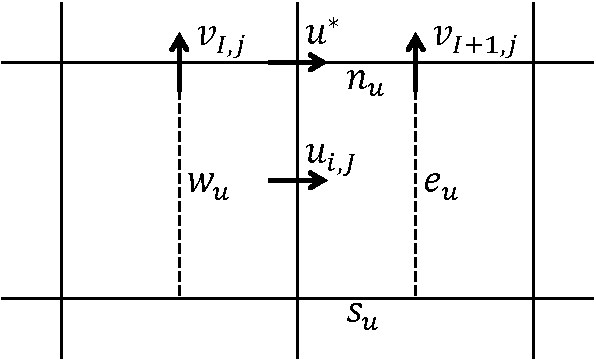
\includegraphics[width=0.6\textwidth]{lateral_adv_flux_black.pdf}
		\caption[Degrees of freedom involved in the lateral part of the 
		advective flux]{Degrees of freedom involved in the lateral part of the 
		advective flux.}
		\label{fig:lat_adv_flux}
	\end{figure}
\end{itemize}
The equation for the component $v$ of the velocity is analogous to the one for 
$u$ described above, with the only addition of the gravity term:
\begin{equation}
\frac{\partial v}{\partial t} + \nabla \cdot (v \mathbf{v}) - \nabla \cdot 
(\nu_\text{eff} \nabla v) + \frac{1}{\varrho}\frac{\partial}{\partial y} \big(p 
+ \varrho k\big) - g= 0,
\end{equation}
with $g = \SI{-9.81}{m/s}$. The gravity term is discretized straight-forward:
\begin{equation}
\int_{V_v} g \; dV = g |V_v|,
\end{equation}
where $V_v = [x_{i-1}, xi] \times [y_J, y_{J+1}]$ is the ``blue'' control 
volume in 
Figure~\ref{fig:staggrid}. 

%
\subsection{Differencing schemes} \label{subsec:diffscheme} %Linear 
%differencing schemes ?
The choice of the scheme for the approximation of a transported field is of 
great importance for both the accuracy and the stability of the solution of the 
problem. In general this decision has to be taken for every convective term, 
indeed we have found it both in the discretization of the velocity 
equation and of the turbulence model equations. As already mentioned, an 
important property that the scheme should have is the \emph{transportativeness} 
(see \cite{main:vermal}), i.e. it should take into account the direction of the 
flow. From a physical point of view this comes from the fact that, when in a 
flow convection is dominating over diffusion, a bias of the value on the face 
towards the direction where the flow comes from must occur. From a mathematical 
point of view instead we can introduce the following \emph{Péclet number}
\begin{equation}
	Pe = \frac{|u| h}{2\nu},
\end{equation}
where $h$ denotes the cell width. When the grid is too coarse or the viscosity 
is too low $Pe\rightarrow\infty$, and this can lead to a lost of stability of 
the numerical method (see for example \cite{main:quarteroni}).

In the following we will list the most immediate options, referring to the 
convective term of the equation~\eqref{eq:stagu} for the $x$-component of the 
velocity. It is considered here the case of a uniform grid, with positive 
transporting velocity according to 
Figure~\ref{fig:superscripts}, but all the schemes can be generalized to the 
case of non-uniform grids. Moreover the basic construction is one-dimensional, 
so it can be used for every dimension also in a multi-dimensional problem. For 
a complete description see for example in \cite{main:vermal}.
\begin{figure}
	\centering
	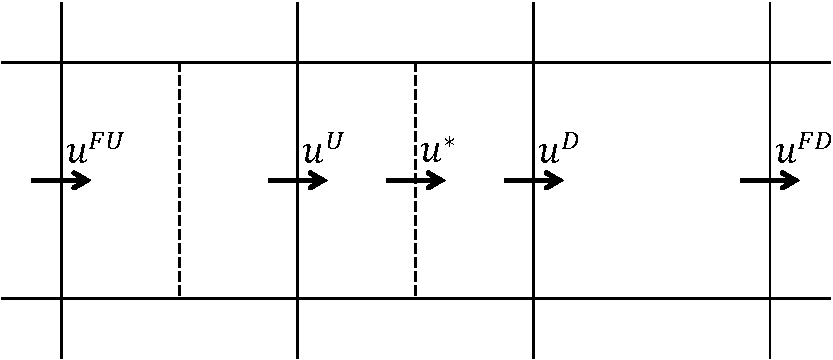
\includegraphics[width=0.75\textwidth]{trecelle_black.pdf}
	\caption[Location of the degrees of freedom used to approximate 
	$u^*$]{Location of the degrees of freedom used to approximate $u^*$. The 
	superscripts $^U$, $^{FU}$, $^D$ and $^{FD}$ stand respectively for 
	upstream, far-upstream, downstream and far-downstream. They hold for the 
	case of positive transporting velocity at the face where $u^*$ is.}
	\label{fig:superscripts}
\end{figure}
\subsubsection{CD scheme}
The Central Differencing (CD) scheme consists in using an average between the 
two first neighbouring values:
\begin{equation} \label{eq:cd}
	u^* = \frac{u^D + u^U}{2}.
\end{equation}
Employing Taylor expansions, it can be easily seen that this approximation is 
of second order, but being symmetric it does not have the transportativeness 
property. Indeed it can be shown that when $Pe > 1$ it is not stable.
%
\subsubsection{Upwind scheme}
In opposition to the CD scheme, the upwind scheme consists in using only the 
upstream value:
\begin{equation}
	u^* = u^U
\end{equation}
It is a simple, widely used and robust scheme as it has the transportativeness 
property, but its accuracy is only of first order, indeed it introduces in the 
solution an important amount of numerical diffusion that smooths the gradients. 
%
\subsubsection{Hybrid scheme}
The hybrid scheme (\cite{diff:hybrid}) consists in evaluating if $Pe<1$ or 
$Pe>1$ at each face and then employing the CD or the upwind respectively. It 
exploits the good properties of the two schemes mentioned above, so it is 
highly stable and accurate when the diffusion is dominant, however the overall 
accuracy in terms of Taylor expansions reduces to first order.
%
\subsubsection{QUICK scheme}
The Quadratic Upstream Interpolation for Convective Kinetics (QUICK) scheme 
(\cite{fv:leonard}) is an higher-order method that involves an extended stencil 
of degrees of freedom. It can be obtained evaluating the quadratic interpolator 
of $u^D$, $u^U$ and 
$u^{FU}$ at the position where $u^*$ is:
\begin{equation} \label{eq:quick}
	u^* = \frac{3u^D + 6u^U - u^{FU}}{8}.
\end{equation}
Its accuracy is of third order, but it may produce unphysical overshoots or 
undershoots in the solution when there are strong gradients. This behaviour is 
not desirable, in particular in the case where the simulation involves 
quantities such as the turbulent kinetic energy $k$ that have to be positive. 
%
\subsubsection{LUD scheme}
The Linear Upwind Differencing (LUD) scheme is an extension of the upwind 
scheme that has a second order accuracy, however it can produce too unphysical 
oscillations. It can be obtained evaluating the linear interpolator of $u^U$ 
and 
$u^{FU}$ at the position where $u^*$ is:
\begin{equation} \label{eq:lud}
u^* = \frac{3u^U - u^{FU}}{2}
\end{equation}
%
\subsubsection{An example}
We can see the behaviour of the CD, Upwind and QUICK methods when they are 
applied to a one-dimensional scalar conservation law:
\begin{align}
	\label{eq:1dconslaw} \frac{\partial \phi}{\partial t} + \frac{\partial 
	\phi}{\partial x} = 0, 
	\quad &\forall x \in (0, 1), \; \forall t > 0\\
	\phi(0, t) = 1, \quad &\forall t>0\\
	\label{eq:1dconslawend}\phi(x, 0) = 0, \quad &\forall x \in (0,1)
\end{align}
In this case there is no diffusion but only the linear transport of a step from 
left to right. The equation~\eqref{eq:1dconslaw} can be discretized with finite 
volumes storing the degrees of freedom at the ends of each cells, as it is in 
the staggered grid concept. Then the differencing schemes presented above can 
be applied to the discretization of the transport term, while for the temporal 
discretization we can use the Backward Euler method (see 
Subsection~\ref{subsec:time}).
\begin{figure}[t]
	\centering
	% This file was created by matlab2tikz.
%
\definecolor{mycolor1}{rgb}{0.00000,0.44700,0.74100}%
\definecolor{mycolor2}{rgb}{0.85000,0.32500,0.09800}%
\definecolor{mycolor3}{rgb}{0.92900,0.69400,0.12500}%
\definecolor{mycolor4}{rgb}{0.49400,0.18400,0.55600}%
%
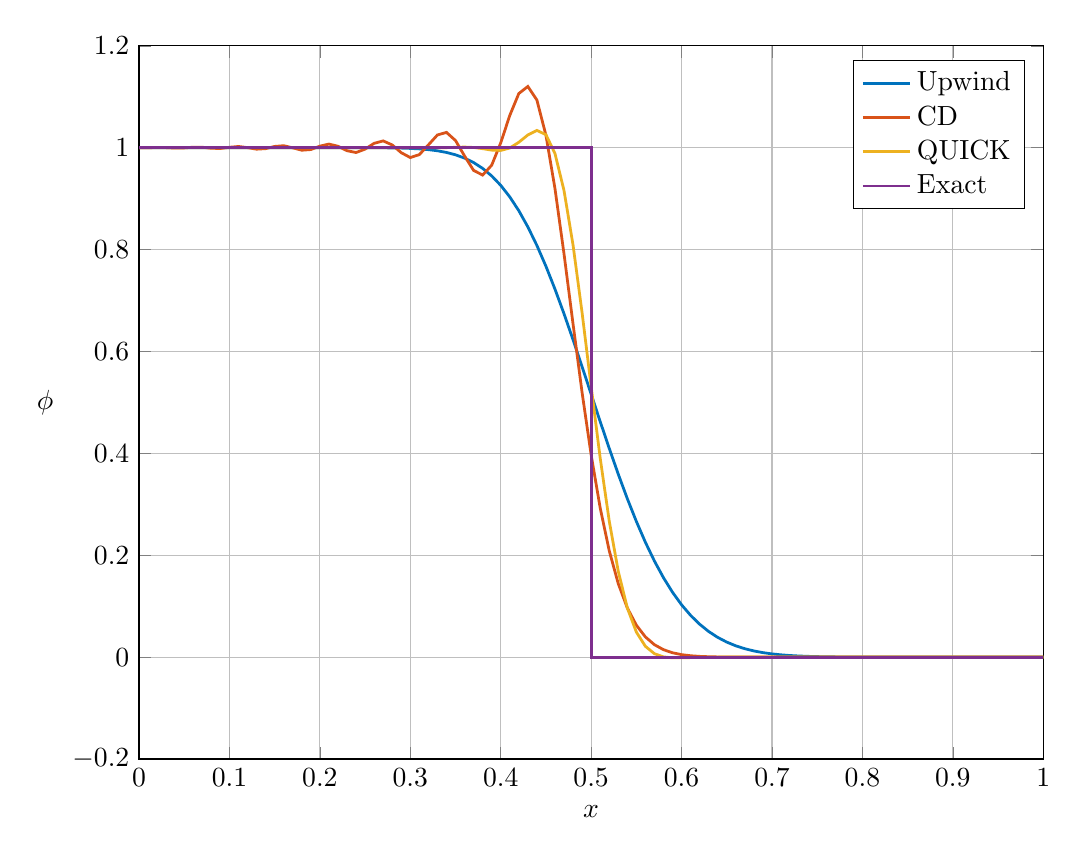
\begin{tikzpicture}

\begin{axis}[%
width=4.521in,
height=3.566in,
at={(0.758in,0.481in)},
scale only axis,
xmin=0,
xmax=1,
xlabel={$x$},
ymin=-0.2,
ymax=1.2,
ylabel style={rotate=-90},
ylabel={$\phi$},
axis background/.style={fill=white},
xmajorgrids,
ymajorgrids,
legend style={legend cell align=left, align=left}
]
\addplot [color=mycolor1, line width=1.0pt]
  table[row sep=crcr]{%
0	1\\
0.01	0.999999999999998\\
0.02	0.999999999999996\\
0.03	0.999999999999994\\
0.04	0.999999999999992\\
0.05	0.999999999999989\\
0.06	0.999999999999986\\
0.07	0.99999999999996\\
0.08	0.999999999999793\\
0.09	0.999999999998831\\
0.1	0.999999999993898\\
0.11	0.999999999971067\\
0.12	0.999999999874841\\
0.13	0.999999999502328\\
0.14	0.999999998168577\\
0.15	0.999999993725629\\
0.16	0.999999979885173\\
0.17	0.999999939386113\\
0.18	0.999999827634698\\
0.19	0.999999535839338\\
0.2	0.999998812633614\\
0.21	0.999997106525567\\
0.22	0.999993265936024\\
0.23	0.999984997559364\\
0.24	0.999967937904754\\
0.25	0.999934141695054\\
0.26	0.999869744553662\\
0.27	0.999751533017892\\
0.28	0.999542175213802\\
0.29	0.999183955854206\\
0.3	0.998591041052117\\
0.31	0.997640580657252\\
0.32	0.996163325498081\\
0.33	0.993934852516489\\
0.34	0.990668881094432\\
0.35	0.986014435190807\\
0.36	0.979558658275129\\
0.37	0.970836838452181\\
0.38	0.959350608906481\\
0.39	0.944594376212604\\
0.4	0.926088890922847\\
0.41	0.903419671442894\\
0.42	0.876276925280645\\
0.43	0.844492887025716\\
0.44	0.808072276594065\\
0.45	0.767211963651117\\
0.46	0.722306892457252\\
0.47	0.673940758463859\\
0.48	0.622861630494047\\
0.49	0.569944427843504\\
0.5	0.516143635538314\\
0.51	0.462440662855497\\
0.52	0.409790689637048\\
0.53	0.359073669980816\\
0.54	0.311053438676802\\
0.55	0.266347735122728\\
0.56	0.225410611537675\\
0.57	0.188527326489454\\
0.58	0.15582061757907\\
0.59	0.12726632782502\\
0.6	0.102715798267608\\
0.61	0.0819222436879219\\
0.62	0.064568457451522\\
0.63	0.050293568773193\\
0.64	0.0387171078248224\\
0.65	0.0294592278334407\\
0.66	0.0221565085115676\\
0.67	0.0164732627583193\\
0.68	0.0121086534010078\\
0.69	0.00880018614753774\\
0.7	0.00632428443479598\\
0.71	0.00449468953278292\\
0.72	0.00315938979635853\\
0.73	0.00219669263790105\\
0.74	0.00151093575790394\\
0.75	0.00102821009176346\\
0.76	0.000692350052533607\\
0.77	0.000461345838948479\\
0.78	0.000304252064420694\\
0.79	0.000198607416515645\\
0.8	0.000128339745066717\\
0.81	8.21068112383886e-05\\
0.82	5.20112987575462e-05\\
0.83	3.26260518048084e-05\\
0.84	2.02687530901388e-05\\
0.85	1.24718860439782e-05\\
0.86	7.60197122584152e-06\\
0.87	4.5904488488754e-06\\
0.88	2.74640275388882e-06\\
0.89	1.62816405785874e-06\\
0.9	9.56535504982658e-07\\
0.91	5.5695043665537e-07\\
0.92	3.21430766012914e-07\\
0.93	1.83889140173297e-07\\
0.94	1.04295159237761e-07\\
0.95	5.86479341944607e-08\\
0.96	3.27010904856373e-08\\
0.97	1.80814200246999e-08\\
0.98	9.91523108869357e-09\\
0.99	5.3927683848014e-09\\
1	3.78657525181429e-09\\
};
\addlegendentry{Upwind}

\addplot [color=mycolor2, line width=1.0pt]
  table[row sep=crcr]{%
0	1\\
0.01	0.999965710272451\\
0.02	1.0003711465264\\
0.03	1.00014854307904\\
0.04	0.999270844467522\\
0.05	0.99960061856003\\
0.06	1.00102346309916\\
0.07	1.00086577735392\\
0.08	0.99886995603546\\
0.09	0.998429046767205\\
0.1	1.00083403493599\\
0.11	1.00239038375991\\
0.12	1.00012095987893\\
0.13	0.997070624727386\\
0.14	0.998159339376732\\
0.15	1.00247724177743\\
0.16	1.00390489753821\\
0.17	0.999721043584093\\
0.18	0.995016751203348\\
0.19	0.996388693579341\\
0.2	1.00305748718819\\
0.21	1.0070996420994\\
0.22	1.00283795879653\\
0.23	0.994077686119459\\
0.24	0.990516376643465\\
0.25	0.99720788995073\\
0.26	1.00856755910146\\
0.27	1.01330322516727\\
0.28	1.00533865198346\\
0.29	0.990143473793654\\
0.3	0.980639837378823\\
0.31	0.986428547191385\\
0.32	1.0055054295642\\
0.33	1.02499426078756\\
0.34	1.03002123275231\\
0.35	1.01405329869804\\
0.36	0.98370328084332\\
0.37	0.955361373773731\\
0.38	0.946290123037388\\
0.39	0.965579669516141\\
0.4	1.0095677179787\\
0.41	1.06328348178933\\
0.42	1.10635367292669\\
0.43	1.12018661001756\\
0.44	1.09346505650795\\
0.45	1.0243789005889\\
0.46	0.919640397126949\\
0.47	0.791419977970305\\
0.48	0.65367119674773\\
0.49	0.519030386095064\\
0.5	0.396908803611655\\
0.51	0.292845366943997\\
0.52	0.208828815737963\\
0.53	0.144163960111455\\
0.54	0.0964932311582958\\
0.55	0.0627076139101309\\
0.56	0.0396176304571858\\
0.57	0.0243623166423223\\
0.58	0.0145977859589567\\
0.59	0.00853165663445841\\
0.6	0.00486815225843776\\
0.61	0.00271428768884109\\
0.62	0.0014799878436374\\
0.63	0.000789762153221659\\
0.64	0.000412737425771835\\
0.65	0.000211385129457051\\
0.66	0.000106160712960325\\
0.67	5.23108205197296e-05\\
0.68	2.53041786042231e-05\\
0.69	1.20222887601928e-05\\
0.7	5.6128716363789e-06\\
0.71	2.57622411591923e-06\\
0.72	1.16297368003659e-06\\
0.73	5.16560761864122e-07\\
0.74	2.25843172929901e-07\\
0.75	9.72270535293513e-08\\
0.76	4.12301492874685e-08\\
0.77	1.72280576588568e-08\\
0.78	7.09562783110579e-09\\
0.79	2.88145498743889e-09\\
0.8	1.15405650598619e-09\\
0.81	4.55993814246403e-10\\
0.82	1.77797204740791e-10\\
0.83	6.84286241215848e-11\\
0.84	2.60019559804264e-11\\
0.85	9.75739490100953e-12\\
0.86	3.616777968438e-12\\
0.87	1.32454500734859e-12\\
0.88	4.79360068971018e-13\\
0.89	1.71473634698169e-13\\
0.9	6.06401463557598e-14\\
0.91	2.12048214707643e-14\\
0.92	7.33334019249338e-15\\
0.93	2.50865286932442e-15\\
0.94	8.49038192920412e-16\\
0.95	2.84337363183936e-16\\
0.96	9.42429903646218e-17\\
0.97	3.09084521166096e-17\\
0.98	1.00693670408514e-17\\
0.99	3.14077517289222e-18\\
1	1.30466238536566e-18\\
};
\addlegendentry{CD}

\addplot [color=mycolor3, line width=1.0pt]
  table[row sep=crcr]{%
0	1\\
0.01	0.999999999995262\\
0.02	1.00000000004294\\
0.03	0.9999999999912\\
0.04	0.99999999978397\\
0.05	1.00000000007817\\
0.06	1.00000000078217\\
0.07	0.999999999738437\\
0.08	0.999999997478595\\
0.09	1.00000000044043\\
0.1	1.00000000758953\\
0.11	1.00000000077066\\
0.12	0.999999978722831\\
0.13	0.999999989546124\\
0.14	1.00000005365586\\
0.15	1.00000005558989\\
0.16	0.999999888198641\\
0.17	0.999999783023942\\
0.18	1.00000014365421\\
0.19	1.00000066917569\\
0.2	1.00000016879789\\
0.21	0.999998441135465\\
0.22	0.999998136214366\\
0.23	1.00000208086011\\
0.24	1.00000680693682\\
0.25	1.00000234725487\\
0.26	0.999986008302737\\
0.27	0.999977192386767\\
0.28	1.00000468433908\\
0.29	1.0000611995447\\
0.3	1.00007464548147\\
0.31	0.999963804672798\\
0.32	0.999768474427161\\
0.33	0.999717492876302\\
0.34	1.0000740864123\\
0.35	1.00078152688761\\
0.36	1.00121594040801\\
0.37	1.00044548221478\\
0.38	0.998081689000521\\
0.39	0.995224889179441\\
0.4	0.994620035501864\\
0.41	0.999393171277525\\
0.42	1.01062375269566\\
0.43	1.02497613745603\\
0.44	1.03394302606178\\
0.45	1.02559975158592\\
0.46	0.988454410759239\\
0.47	0.915793052889107\\
0.48	0.808577592237637\\
0.49	0.675636328584134\\
0.5	0.531162002238621\\
0.51	0.390681264237169\\
0.52	0.267129177339398\\
0.53	0.168344132852575\\
0.54	0.0964975297312753\\
0.55	0.0491554716101291\\
0.56	0.0211897918605249\\
0.57	0.00671289177835233\\
0.58	0.000482493061530729\\
0.59	-0.0014066429442749\\
0.6	-0.00143498240798926\\
0.61	-0.000929732816774027\\
0.62	-0.000455118195225722\\
0.63	-0.000161407874156621\\
0.64	-2.54614459088232e-05\\
0.65	1.75654911986119e-05\\
0.66	2.03641743786821e-05\\
0.67	1.23082448611261e-05\\
0.68	5.110132501568e-06\\
0.69	1.23558886770601e-06\\
0.7	-1.68399632307439e-07\\
0.71	-3.89521164225457e-07\\
0.72	-2.51907941517708e-07\\
0.73	-1.02706380241783e-07\\
0.74	-2.24857631892333e-08\\
0.75	4.57658242611726e-09\\
0.76	7.56691986686351e-09\\
0.77	4.29278769841257e-09\\
0.78	1.46170982216117e-09\\
0.79	1.72039443552797e-10\\
0.8	-1.55346555440935e-10\\
0.81	-1.31647173167267e-10\\
0.82	-5.64411371340995e-11\\
0.83	-1.24899207153375e-11\\
0.84	1.9906596373481e-12\\
0.85	3.35824693909456e-12\\
0.86	1.70700405002962e-12\\
0.87	4.67687981928616e-13\\
0.88	-2.23227565065507e-15\\
0.89	-7.70766789518374e-14\\
0.9	-4.44186596934674e-14\\
0.91	-1.33448697541153e-14\\
0.92	-6.52923800100817e-16\\
0.93	1.69069287314303e-15\\
0.94	1.0405244781143e-15\\
0.95	3.18554261065671e-16\\
0.96	1.87786792697895e-17\\
0.97	-3.6768924328292e-17\\
0.98	-2.23805157994266e-17\\
0.99	-6.58055008490752e-18\\
1	-4.00561578240812e-19\\
};
\addlegendentry{QUICK}

\addplot [color=mycolor4, line width=1.0pt]
  table[row sep=crcr]{%
0	1\\
0.5	1\\
0.5	0\\
1	0\\
};
\addlegendentry{Exact}

\end{axis}
\end{tikzpicture}%
	\caption[Solution of a one-dimensional scalar conservation law]{Solution of 
	the problem \eqref{eq:1dconslaw}--\eqref{eq:1dconslawend} at the time 
	$t=0.5$. The upwind method smooths the gradient, while the CD and QUICK 
	methods produce oscillations.}
	\label{fig:1dconslaw}
\end{figure}

In Figure~\ref{fig:1dconslaw} we can see the solution at $t=0.5$. The upwind 
method is very diffusive near the step, but bounded within the extrema of the 
exact solution. The CD and QUICK methods instead approximate better the steep 
gradient, but produce oscillations for $x<0.5$.
%
\subsection{TVD methods} \label{subsec:tvd}
Total Variation Diminishing (TVD) methods are part of a category of methods 
called \emph{high resolution methods}, that address the problem of having a 
solution without any oscillation and with an higher order accuracy, second 
order in this case. They were originally developed for scalar conservation laws 
of the type:
\begin{align}
	\label{eq:conslaw} &\frac{\partial \phi}{\partial t} + \frac{\partial f(x) 
	}{\partial x} = 0. 
%\quad t>0 \quad x 
%	\in 
%	\mathbb{R}\\[1ex]
%	\label{eq:conslawic} &\phi(x, 0) = \phi_0(x), \quad x \in \mathbb{R}
\end{align}

For this kind of problem the \emph{total variation} of the numerical solution 
can be defined as:
\begin{equation}
	TV(\phi) = \sum_{i=1}^{N_\text{dof}-1} |\phi_{i+1} - \phi_i|,
\end{equation}
where $\phi_i$ is the numerical solution at the node $i$ of the discretized 
domain. Then a method is called \emph{TVD} if the total variation of the 
solution does not increase with time, i.e. 
\begin{equation}\label{eq:tvdcondition}
	TV(\phi ^{n+1}) \leq TV(\phi^n) \quad \forall n>0,
\end{equation}
where $\phi^n$ is the numerical solution at the time-step $t^n$. In 
\cite{tvd:monotonicity} it has been proved that a TVD scheme is 
\emph{monotonicity preserving}, i.e. it does not create new 
local extrema, local minima are non-decreasing and local maxima are 
non-increasing. This is the desirable property that we would like to have in 
order avoid the development of solutions containing overshoots and undershoots, 
as it can happen using the higher order methods presented in the previous 
subsection.

According to \cite{tvd:sweeby} and \cite{main:darwish} we can achieve our 
target adding to the first order upwind approximation a second order 
non-linear 
anti-diffusive flux: 
\begin{equation} \label{eq:tvdformula}
u^* = u^U + \frac{1}{2}\psi(r)(u^D - u^U), \quad r = 
\frac{u^U - u^{FU}}{u^D - u^U}.
\end{equation}
The flux includes a function $\psi(r)$ called \emph{flux limiter}, that should 
dampen the second order contribution in regions of the domain where it could 
produces oscillations. It is chosen non-negative in order to preserve the sign 
of the flux and it depends on the variable $r$, that is defined as the ratio 
between two consecutive differences of the solution. The non-linearity can not 
be avoided, indeed it was proved by \textcite{tvd:godunov} that any 
monotonicity preserving linear scheme can be at most first order accurate.

Exploiting the approximation \eqref{eq:tvdformula} to solve a problem like
\eqref{eq:conslaw} and imposing the TVD condition \eqref{eq:tvdcondition} on 
the solution, we obtain the following bounds for the flux limiter function:
\begin{align}
\notag \psi(r) = 0 \quad &\text{if} \quad r < 0\\
\psi(r) \leq \min \{2r, 1\} \quad &\text{if} \quad 0 \leq r \leq 1\\
\notag \psi(r) \leq 2 \quad &\text{if} \quad r > 2
\end{align}
Notice that when $r<0$ we are in presence of a local maximum or minimum, 
because it means that the difference between the upstream and downstream nodes 
has opposite sign of the difference between the far upstream and upstream 
nodes. In this $\psi$ is set to zero, so only the first order upwind 
contribution is employed in the approximation of $u^*$.
It is also required to $\psi$ the following symmetry property:
\begin{equation}
\frac{\psi(r)}{r} = \psi\bigg(\frac{1}{r}\bigg),
\end{equation}
that ensures that backward- and forward-facing gradients are treated in the 
same way.

In order to have a second order scheme, $\psi$ must be at least 
Lipschitz-continuous. Moreover, following \cite{tvd:sweeby} and 
\cite{tvd:vanleer}, any second order scheme 
can be obtained as a convex combination of the CD scheme \eqref{eq:cd} and the 
LUD scheme \eqref{eq:lud} in the following way:
\begin{equation}
	\psi(r) = \theta(r) \psi_{CD}(r) + (1-\theta(r))\psi_{LUD}(r) \quad \forall 
	r >0,
\end{equation}
where $\theta(r)$ is a parameter such that $0 \leq \theta(r) \leq 1,\; \forall 
r>0$, while $\psi_{CD}$ and $\psi_{LUD}$ are the linear flux limiter functions 
that can be associated to the schemes CD and LUD rearranging the 
approximations \eqref{eq:cd} and \eqref{eq:lud}:
\begin{gather}
	\psi_{CD}(r) = 1 \quad \forall r,\\
	\psi_{LUD}(r) = r \quad \forall r.
\end{gather}

Thus, adding these requirements to the previous ones, we 
obtain the following bounds for the flux limiter function of a TVD method:
\begin{align}
\psi(r) = 0 \quad &\text{if} \quad r < 0 \notag \\
\label{tvd:bounds} r \leq \psi(r) \leq \min \{2r, 1\} \quad &\text{if} \quad 0 
\leq r \leq 1\\
1 \leq \psi(r) \leq \min \{r, 2 \} \quad &\text{if} \quad r > 2 \notag
\end{align}
In Figure~\ref{fig:tvdregion} they are reported in a $\psi-r$ diagram known 
also as Sweby's diagram.
\begin{figure}
	\centering
	% This file was created by matlab2tikz.
%
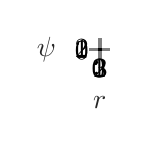
\begin{tikzpicture}

\begin{axis}[%
width=0.951\widthsette,
height=0.68\widthsette,
scale only axis,
xmin=0,
xmax=3.5,
xlabel style={font=\color{white!15!black}},
xlabel={$r$},
ymin=0,
ymax=2.5,
ylabel style={font=\color{white!15!black}, rotate=-90},
ylabel={$\psi$},
axis background/.style={fill=white},
xmajorgrids,
ymajorgrids,
]

\addplot[area legend, draw=black, fill=white!80!black, fill opacity=0.5, forget plot, line width=1pt]
table[row sep=crcr] {%
x	y\\
0	0\\
1	1\\
0.5	1\\
}--cycle;

\addplot[area legend, draw=black, fill=white!80!black, fill opacity=0.5, forget plot, line width=1pt]
table[row sep=crcr] {%
x	y\\
1	1\\
5.5	1\\
5.5	2\\
2	2\\
}--cycle;

\end{axis}
\end{tikzpicture}%
	\caption[The TVD region (Sweby's diagram)]{In grey the TVD region in which 
	the flux 
	limiter functions must fit. It is called also Sweby's diagram.}
	\label{fig:tvdregion}
\end{figure}
% A livello teorico potrei aggiungere la dimostrazione di monotonicity->TVD, 
%l'applicazione di TVD per ottenere i bounds e l'applicazione dei bounds 
%all'approssimazione col flux limiter (come in sweby o in darwish). Potrei 
%mettere qualcosa nell'appendice.
\subsubsection{Flux limters}
Starting from the bounds \eqref{tvd:bounds}, it is easy to create a 
flux limiter function, indeed in literature many possible choices can be 
found. 
We list here some of the most popular functions that have been implemented in 
\DUMUX and in Figure~\ref{fig:fluxlimiters} we can see their graph in the 
Sweby's diagram:
\begin{itemize}
	\item Van Leer \cite{tvd:vanleer}
	\begin{equation} \label{eq:vl}
	\psi(r) = \frac{r+|r|}{1+r}.
	\end{equation}
	It is a smooth function that asymptotically reaches 2 for $r \rightarrow 
	\infty$.
%
	\item Van Alabada \cite{tvd:vanalabada}
	\begin{equation}
	\psi(r)=
	\begin{cases}
	\dfrac{r^2+r}{r^2+1} \quad &\text{if $r\geq 0$}\\[2ex]
	0 \quad &\text{if $r<0$}
	\end{cases}
	\end{equation}
	It is a smooth function that instead goes to 1 as $r \rightarrow \infty$.
%
	\item Min-Mod \cite{tvd:roe}
	\begin{equation}
	\psi(r) = \max \{0, \min \{ r,1\} \}
	\end{equation}
	It is a piecewise linear function that lies on the lower boundary of the 
	TVD region. Intuitively, using this limiter we add to the upstream value  
	half of	the smallest increment in absolute value between $u^U-u^{FU}$ and 
	$u^D - u^U$.
%
	\item Superbee \cite{tvd:roe}
	\begin{equation}
	\psi(r)=\max \{0, \min \{ 2r, 1\}, \min \{ r, 2\} \}
	\end{equation}
	It is a piecewise linear function that lies on the upper boundary of the 
	TVD region.
%
	\item UMIST \cite{tvd:lien}
	\begin{equation}
	\psi(r)=\max \bigg\{0, \min \bigg\{ 2r, \frac{3r+1}{4},\frac{r+3}{4}, 
	2\bigg\} \bigg\}
	\end{equation}
	It is a piecewise linear function that was designed as a symmetrical TVD 
	version of QUICK.
%
	\item MC (Monotinized Central) limiter \cite{tvd:mclimiter}
	\begin{equation}
	\psi(r)=\max \bigg\{0, \min \bigg\{ 2r, \frac{r+1}{2}, 2\bigg\} \bigg\}
	\end{equation}
	It is also known as MUSCL (Monotonic Upstream-Centred Scheme for 
	Conservation Laws) limiter.
%	
%	\item WAHYD \cite{nonunif:hou}
%	\begin{equation}
%	\psi(r)=
%	\begin{cases}
%	\dfrac{r + |r|}{r + 1} & \text{if $r \leq 1$} \\[2ex]
%	\min \bigg\{ \dfrac{r + 2 r^2}{2 + r^2}, 2 \bigg\} & \text{if $r>1$}
%	\end{cases}
%	\end{equation}
%	It is a hybrid scheme, for $r\leq 1$ it is the Van Leer scheme 
%	\eqref{eq:vl}, while for $r>1$ it is closer to the upper bound of the TVD 
%	region.
\end{itemize}
\begin{figure}[t]
	\centering
	% This file was created by matlab2tikz.
%
\definecolor{mycolor1}{rgb}{0.92900,0.69400,0.12500}%
\definecolor{mycolor2}{rgb}{0.49400,0.18400,0.55600}%
\definecolor{mycolor3}{rgb}{0.46600,0.67400,0.18800}%
\definecolor{mycolor4}{rgb}{0.30100,0.74500,0.93300}%
\definecolor{mycolor5}{rgb}{0.63500,0.07800,0.18400}%
\definecolor{mycolor6}{rgb}{0.00000,0.44700,0.74100}%
%
\begin{tikzpicture}

\begin{axis}[%
width=4.521in,
height=3.566in,
at={(0.758in,0.481in)},
scale only axis,
xmin=0,
xmax=5.5,
xlabel={$r$},
ymin=0,
ymax=3,
ylabel style={rotate=-90},
ylabel={$\psi$},
axis background/.style={fill=white},
xmajorgrids,
ymajorgrids,
legend style={at={(0.03,0.97)}, anchor=north west, legend cell align=left, align=left}
]

\addplot[area legend, draw=none, fill=white!95!black, fill opacity=0.5, forget plot]
table[row sep=crcr] {%
x	y\\
0	0\\
1	1\\
0.5	1\\
}--cycle;

\addplot[area legend, draw=none, fill=white!95!black, fill opacity=0.5, forget plot]
table[row sep=crcr] {%
x	y\\
1	1\\
5.5	1\\
5.5	2\\
2	2\\
}--cycle;
\addplot [color=mycolor1, line width=1.0pt]
  table[row sep=crcr]{%
0	0\\
0.05	0.0952380952380952\\
0.1	0.181818181818182\\
0.15	0.260869565217391\\
0.2	0.333333333333333\\
0.25	0.4\\
0.3	0.461538461538462\\
0.35	0.518518518518518\\
0.4	0.571428571428572\\
0.45	0.620689655172414\\
0.5	0.666666666666667\\
0.55	0.709677419354839\\
0.6	0.75\\
0.65	0.787878787878788\\
0.7	0.823529411764706\\
0.75	0.857142857142857\\
0.8	0.888888888888889\\
0.85	0.918918918918919\\
0.9	0.947368421052632\\
0.95	0.974358974358974\\
1	1\\
1.05	1.02439024390244\\
1.1	1.04761904761905\\
1.15	1.06976744186047\\
1.2	1.09090909090909\\
1.25	1.11111111111111\\
1.3	1.1304347826087\\
1.35	1.14893617021277\\
1.4	1.16666666666667\\
1.45	1.18367346938776\\
1.5	1.2\\
1.55	1.2156862745098\\
1.6	1.23076923076923\\
1.65	1.24528301886792\\
1.7	1.25925925925926\\
1.75	1.27272727272727\\
1.8	1.28571428571429\\
1.85	1.29824561403509\\
1.9	1.31034482758621\\
1.95	1.32203389830508\\
2	1.33333333333333\\
2.05	1.34426229508197\\
2.1	1.35483870967742\\
2.15	1.36507936507937\\
2.2	1.375\\
2.25	1.38461538461538\\
2.3	1.39393939393939\\
2.35	1.40298507462687\\
2.4	1.41176470588235\\
2.45	1.42028985507246\\
2.5	1.42857142857143\\
2.55	1.43661971830986\\
2.6	1.44444444444444\\
2.65	1.45205479452055\\
2.7	1.45945945945946\\
2.75	1.46666666666667\\
2.8	1.47368421052632\\
2.85	1.48051948051948\\
2.9	1.48717948717949\\
2.95	1.49367088607595\\
3	1.5\\
3.05	1.50617283950617\\
3.1	1.51219512195122\\
3.15	1.51807228915663\\
3.2	1.52380952380952\\
3.25	1.52941176470588\\
3.3	1.53488372093023\\
3.35	1.54022988505747\\
3.4	1.54545454545455\\
3.45	1.55056179775281\\
3.5	1.55555555555556\\
3.55	1.56043956043956\\
3.6	1.56521739130435\\
3.65	1.56989247311828\\
3.7	1.57446808510638\\
3.75	1.57894736842105\\
3.8	1.58333333333333\\
3.85	1.58762886597938\\
3.9	1.59183673469388\\
3.95	1.5959595959596\\
4	1.6\\
4.05	1.6039603960396\\
4.1	1.6078431372549\\
4.15	1.61165048543689\\
4.2	1.61538461538462\\
4.25	1.61904761904762\\
4.3	1.62264150943396\\
4.35	1.62616822429907\\
4.4	1.62962962962963\\
4.45	1.63302752293578\\
4.5	1.63636363636364\\
4.55	1.63963963963964\\
4.6	1.64285714285714\\
4.65	1.64601769911504\\
4.7	1.64912280701754\\
4.75	1.65217391304348\\
4.8	1.6551724137931\\
4.85	1.65811965811966\\
4.9	1.66101694915254\\
4.95	1.66386554621849\\
5	1.66666666666667\\
5.05	1.66942148760331\\
5.1	1.67213114754098\\
5.15	1.67479674796748\\
5.2	1.67741935483871\\
5.25	1.68\\
5.3	1.68253968253968\\
5.35	1.68503937007874\\
5.4	1.6875\\
5.45	1.68992248062016\\
5.5	1.69230769230769\\
};
\addlegendentry{Van Leer}

\addplot [color=mycolor2, line width=1.0pt]
  table[row sep=crcr]{%
0	0\\
0.05	0.0523690773067332\\
0.1	0.108910891089109\\
0.15	0.168704156479218\\
0.2	0.230769230769231\\
0.25	0.294117647058824\\
0.3	0.357798165137615\\
0.35	0.420935412026726\\
0.4	0.482758620689655\\
0.45	0.542619542619542\\
0.5	0.6\\
0.55	0.654510556621881\\
0.6	0.705882352941177\\
0.65	0.753954305799649\\
0.7	0.798657718120805\\
0.75	0.84\\
0.8	0.878048780487805\\
0.85	0.912917271407838\\
0.9	0.94475138121547\\
0.95	0.973718791064389\\
1	1\\
1.05	1.02378121284185\\
1.1	1.04524886877828\\
1.15	1.06458557588805\\
1.2	1.08196721311475\\
1.25	1.09756097560976\\
1.3	1.11152416356877\\
1.35	1.12400354295837\\
1.4	1.13513513513514\\
1.45	1.1450443190975\\
1.5	1.15384615384615\\
1.55	1.16164584864071\\
1.6	1.1685393258427\\
1.65	1.17461383478845\\
1.7	1.17994858611825\\
1.75	1.18461538461538\\
1.8	1.18867924528302\\
1.85	1.19219898247598\\
1.9	1.19522776572668\\
1.95	1.19781363872983\\
2	1.2\\
2.05	1.20182604517059\\
2.1	1.20332717190388\\
2.15	1.20453534904402\\
2.2	1.20547945205479\\
2.25	1.20618556701031\\
2.3	1.20667726550079\\
2.35	1.20697585281717\\
2.4	1.20710059171598\\
2.45	1.20706890396287\\
2.5	1.20689655172414\\
2.55	1.20659780073309\\
2.6	1.20618556701031\\
2.65	1.20567154876909\\
2.7	1.20506634499397\\
2.75	1.2043795620438\\
2.8	1.20361990950226\\
2.85	1.20279528637983\\
2.9	1.201912858661\\
2.95	1.20097912909044\\
3	1.2\\
3.05	1.19898082989566\\
3.1	1.19792648444863\\
3.15	1.19684138246738\\
3.2	1.19572953736655\\
3.25	1.19459459459459\\
3.3	1.19343986543314\\
3.35	1.19226835753733\\
3.4	1.19108280254777\\
3.45	1.18988568106956\\
3.5	1.18867924528302\\
3.55	1.1874655394229\\
3.6	1.18624641833811\\
3.65	1.18502356432187\\
3.7	1.18379850238257\\
3.75	1.18257261410788\\
3.8	1.18134715025907\\
3.85	1.18012324221836\\
3.9	1.17890191239975\\
3.95	1.17768408372233\\
4	1.17647058823529\\
4.05	1.17526217497486\\
4.1	1.17405951712521\\
4.15	1.1728632185485\\
4.2	1.17167381974249\\
4.25	1.17049180327869\\
4.3	1.1693175987686\\
4.35	1.16815158740118\\
4.4	1.16699410609037\\
4.45	1.16584545126788\\
4.5	1.16470588235294\\
4.55	1.163575624928\\
4.6	1.16245487364621\\
4.65	1.16134379489446\\
4.7	1.16024252923343\\
4.75	1.15915119363395\\
4.8	1.15806988352745\\
4.85	1.15699867468651\\
4.9	1.15593762495002\\
4.95	1.15488677580629\\
5	1.15384615384615\\
5.05	1.15281577209697\\
5.1	1.15179563124769\\
5.15	1.15078572077391\\
5.2	1.14978601997147\\
5.25	1.14879649890591\\
5.3	1.14781711928498\\
5.35	1.14684783526036\\
5.4	1.14588859416446\\
5.45	1.14493933718753\\
5.5	1.144\\
};
\addlegendentry{Van Alabada}

\addplot [color=mycolor3, line width=1.0pt]
  table[row sep=crcr]{%
0	0\\
0.05	0.05\\
0.1	0.1\\
0.15	0.15\\
0.2	0.2\\
0.25	0.25\\
0.3	0.3\\
0.35	0.35\\
0.4	0.4\\
0.45	0.45\\
0.5	0.5\\
0.55	0.55\\
0.6	0.6\\
0.65	0.65\\
0.7	0.7\\
0.75	0.75\\
0.8	0.8\\
0.85	0.85\\
0.9	0.9\\
0.95	0.95\\
1	1\\
1.05	1\\
1.1	1\\
1.15	1\\
1.2	1\\
1.25	1\\
1.3	1\\
1.35	1\\
1.4	1\\
1.45	1\\
1.5	1\\
1.55	1\\
1.6	1\\
1.65	1\\
1.7	1\\
1.75	1\\
1.8	1\\
1.85	1\\
1.9	1\\
1.95	1\\
2	1\\
2.05	1\\
2.1	1\\
2.15	1\\
2.2	1\\
2.25	1\\
2.3	1\\
2.35	1\\
2.4	1\\
2.45	1\\
2.5	1\\
2.55	1\\
2.6	1\\
2.65	1\\
2.7	1\\
2.75	1\\
2.8	1\\
2.85	1\\
2.9	1\\
2.95	1\\
3	1\\
3.05	1\\
3.1	1\\
3.15	1\\
3.2	1\\
3.25	1\\
3.3	1\\
3.35	1\\
3.4	1\\
3.45	1\\
3.5	1\\
3.55	1\\
3.6	1\\
3.65	1\\
3.7	1\\
3.75	1\\
3.8	1\\
3.85	1\\
3.9	1\\
3.95	1\\
4	1\\
4.05	1\\
4.1	1\\
4.15	1\\
4.2	1\\
4.25	1\\
4.3	1\\
4.35	1\\
4.4	1\\
4.45	1\\
4.5	1\\
4.55	1\\
4.6	1\\
4.65	1\\
4.7	1\\
4.75	1\\
4.8	1\\
4.85	1\\
4.9	1\\
4.95	1\\
5	1\\
5.05	1\\
5.1	1\\
5.15	1\\
5.2	1\\
5.25	1\\
5.3	1\\
5.35	1\\
5.4	1\\
5.45	1\\
5.5	1\\
};
\addlegendentry{Min-Mod}

\addplot [color=mycolor4, line width=1.0pt]
  table[row sep=crcr]{%
0	0\\
0.05	0.1\\
0.1	0.2\\
0.15	0.3\\
0.2	0.4\\
0.25	0.5\\
0.3	0.6\\
0.35	0.7\\
0.4	0.8\\
0.45	0.9\\
0.5	1\\
0.55	1\\
0.6	1\\
0.65	1\\
0.7	1\\
0.75	1\\
0.8	1\\
0.85	1\\
0.9	1\\
0.95	1\\
1	1\\
1.05	1.05\\
1.1	1.1\\
1.15	1.15\\
1.2	1.2\\
1.25	1.25\\
1.3	1.3\\
1.35	1.35\\
1.4	1.4\\
1.45	1.45\\
1.5	1.5\\
1.55	1.55\\
1.6	1.6\\
1.65	1.65\\
1.7	1.7\\
1.75	1.75\\
1.8	1.8\\
1.85	1.85\\
1.9	1.9\\
1.95	1.95\\
2	2\\
2.05	2\\
2.1	2\\
2.15	2\\
2.2	2\\
2.25	2\\
2.3	2\\
2.35	2\\
2.4	2\\
2.45	2\\
2.5	2\\
2.55	2\\
2.6	2\\
2.65	2\\
2.7	2\\
2.75	2\\
2.8	2\\
2.85	2\\
2.9	2\\
2.95	2\\
3	2\\
3.05	2\\
3.1	2\\
3.15	2\\
3.2	2\\
3.25	2\\
3.3	2\\
3.35	2\\
3.4	2\\
3.45	2\\
3.5	2\\
3.55	2\\
3.6	2\\
3.65	2\\
3.7	2\\
3.75	2\\
3.8	2\\
3.85	2\\
3.9	2\\
3.95	2\\
4	2\\
4.05	2\\
4.1	2\\
4.15	2\\
4.2	2\\
4.25	2\\
4.3	2\\
4.35	2\\
4.4	2\\
4.45	2\\
4.5	2\\
4.55	2\\
4.6	2\\
4.65	2\\
4.7	2\\
4.75	2\\
4.8	2\\
4.85	2\\
4.9	2\\
4.95	2\\
5	2\\
5.05	2\\
5.1	2\\
5.15	2\\
5.2	2\\
5.25	2\\
5.3	2\\
5.35	2\\
5.4	2\\
5.45	2\\
5.5	2\\
};
\addlegendentry{Superbee}

\addplot [color=mycolor5, line width=1.0pt]
  table[row sep=crcr]{%
0	0\\
0.05	0.1\\
0.1	0.2\\
0.15	0.3\\
0.2	0.4\\
0.25	0.5\\
0.3	0.6\\
0.35	0.675\\
0.4	0.7\\
0.45	0.725\\
0.5	0.75\\
0.55	0.775\\
0.6	0.8\\
0.65	0.825\\
0.7	0.85\\
0.75	0.875\\
0.8	0.9\\
0.85	0.925\\
0.9	0.95\\
0.95	0.975\\
1	1\\
1.05	1.025\\
1.1	1.05\\
1.15	1.075\\
1.2	1.1\\
1.25	1.125\\
1.3	1.15\\
1.35	1.175\\
1.4	1.2\\
1.45	1.225\\
1.5	1.25\\
1.55	1.275\\
1.6	1.3\\
1.65	1.325\\
1.7	1.35\\
1.75	1.375\\
1.8	1.4\\
1.85	1.425\\
1.9	1.45\\
1.95	1.475\\
2	1.5\\
2.05	1.525\\
2.1	1.55\\
2.15	1.575\\
2.2	1.6\\
2.25	1.625\\
2.3	1.65\\
2.35	1.675\\
2.4	1.7\\
2.45	1.725\\
2.5	1.75\\
2.55	1.775\\
2.6	1.8\\
2.65	1.825\\
2.7	1.85\\
2.75	1.875\\
2.8	1.9\\
2.85	1.925\\
2.9	1.95\\
2.95	1.975\\
3	2\\
3.05	2\\
3.1	2\\
3.15	2\\
3.2	2\\
3.25	2\\
3.3	2\\
3.35	2\\
3.4	2\\
3.45	2\\
3.5	2\\
3.55	2\\
3.6	2\\
3.65	2\\
3.7	2\\
3.75	2\\
3.8	2\\
3.85	2\\
3.9	2\\
3.95	2\\
4	2\\
4.05	2\\
4.1	2\\
4.15	2\\
4.2	2\\
4.25	2\\
4.3	2\\
4.35	2\\
4.4	2\\
4.45	2\\
4.5	2\\
4.55	2\\
4.6	2\\
4.65	2\\
4.7	2\\
4.75	2\\
4.8	2\\
4.85	2\\
4.9	2\\
4.95	2\\
5	2\\
5.05	2\\
5.1	2\\
5.15	2\\
5.2	2\\
5.25	2\\
5.3	2\\
5.35	2\\
5.4	2\\
5.45	2\\
5.5	2\\
};
\addlegendentry{MC Limiter}

\addplot [color=mycolor6, line width=1.0pt]
  table[row sep=crcr]{%
0	0\\
0.05	0.1\\
0.1	0.2\\
0.15	0.3\\
0.2	0.4\\
0.25	0.4375\\
0.3	0.475\\
0.35	0.5125\\
0.4	0.55\\
0.45	0.5875\\
0.5	0.625\\
0.55	0.6625\\
0.6	0.7\\
0.65	0.7375\\
0.7	0.775\\
0.75	0.8125\\
0.8	0.85\\
0.85	0.8875\\
0.9	0.925\\
0.95	0.9625\\
1	1\\
1.05	1.0125\\
1.1	1.025\\
1.15	1.0375\\
1.2	1.05\\
1.25	1.0625\\
1.3	1.075\\
1.35	1.0875\\
1.4	1.1\\
1.45	1.1125\\
1.5	1.125\\
1.55	1.1375\\
1.6	1.15\\
1.65	1.1625\\
1.7	1.175\\
1.75	1.1875\\
1.8	1.2\\
1.85	1.2125\\
1.9	1.225\\
1.95	1.2375\\
2	1.25\\
2.05	1.2625\\
2.1	1.275\\
2.15	1.2875\\
2.2	1.3\\
2.25	1.3125\\
2.3	1.325\\
2.35	1.3375\\
2.4	1.35\\
2.45	1.3625\\
2.5	1.375\\
2.55	1.3875\\
2.6	1.4\\
2.65	1.4125\\
2.7	1.425\\
2.75	1.4375\\
2.8	1.45\\
2.85	1.4625\\
2.9	1.475\\
2.95	1.4875\\
3	1.5\\
3.05	1.5125\\
3.1	1.525\\
3.15	1.5375\\
3.2	1.55\\
3.25	1.5625\\
3.3	1.575\\
3.35	1.5875\\
3.4	1.6\\
3.45	1.6125\\
3.5	1.625\\
3.55	1.6375\\
3.6	1.65\\
3.65	1.6625\\
3.7	1.675\\
3.75	1.6875\\
3.8	1.7\\
3.85	1.7125\\
3.9	1.725\\
3.95	1.7375\\
4	1.75\\
4.05	1.7625\\
4.1	1.775\\
4.15	1.7875\\
4.2	1.8\\
4.25	1.8125\\
4.3	1.825\\
4.35	1.8375\\
4.4	1.85\\
4.45	1.8625\\
4.5	1.875\\
4.55	1.8875\\
4.6	1.9\\
4.65	1.9125\\
4.7	1.925\\
4.75	1.9375\\
4.8	1.95\\
4.85	1.9625\\
4.9	1.975\\
4.95	1.9875\\
5	2\\
5.05	2\\
5.1	2\\
5.15	2\\
5.2	2\\
5.25	2\\
5.3	2\\
5.35	2\\
5.4	2\\
5.45	2\\
5.5	2\\
};
\addlegendentry{UMIST}

\end{axis}
\end{tikzpicture}%
	\caption[Flux limiter functions]{The Sweby's diagram with the flux limiters 
	presented in this section as functions of $r$.}
	\label{fig:fluxlimiters}
\end{figure}

It is not easy to compare the different flux limiters in order to find the 
best one. Generally the Van Alabada and the Min-Mod can be a bit less accurate 
since $\psi \rightarrow 1$ as $r \rightarrow \infty$, while a scheme like the 
Superbee can produce sharper gradients, but sometimes the convergence can be a 
bit more difficult (it is said to be too compressive). The UMIST instead has a 
more complex function, so its evaluation can be more expensive. However their 
performances should be compared case by case.
%
\subsubsection{Non-uniform grids}
The theory of TVD methods presented above holds for structured grids. In order 
to deal with Cartesian non-uniform grids, that for example employ a grading, we 
have to consider the information about the distances between the degrees of 
freedom involved in the approximation. The generalization however has to be 
consistent, i.e. the approximation~\eqref{eq:tvdformula} has to be recovered in 
case of uniform grid. In literature several slightly different approaches can 
be found, see for example \cite{nonunif:bruner}, \cite{nonunif:darmou}, 
\cite{nonunif:li}, \cite{nonunif:hou}, \cite{nonunif:zeng} and 
\cite{nonunif:berger}. We describe here two of them.

In \cite{nonunif:li}
%
\section{Cell-centred concept}
In the porous-medium region $\Omega_\text{pm}$ we have to solve only a steady 
scalar equation, with the 
pressure as a primary variable, indeed, due to the incompressibility of the 
fluid, the time derivative is not present:
\begin{align}
\label{eq:cellcentred}	\nabla \cdot \mathbf{v} = 0&\\
\label{eq:forch2}	\mathbf{v} + C_F \sqrt{\mathbf{K}} \frac{\varrho}{\mu} 
	|\mathbf{v}|\mathbf{v} + \frac{1}{\mu} \mathbf{K}(\nabla p - \varrho 
	\mathbf{g} ) = \mathbf{0}&
\end{align}
We employ a cell-centred finite volumes method, so the degrees of freedom of 
the pressure are located at the centre of each cell, as we can see in 
Figure~\ref{fig:cellcentred}, and the cells of the grid correspond to the 
control volumes.
\begin{figure}
	\centering
	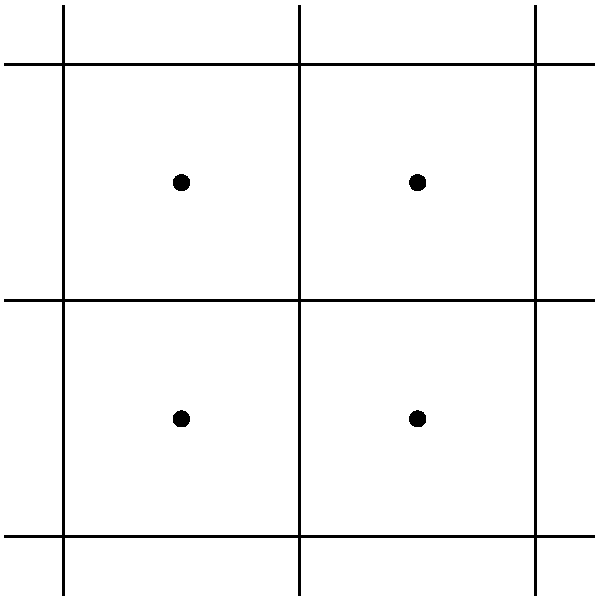
\includegraphics[width=0.4\textwidth]{cellcentred.pdf}
	\caption[Cell-centred grid]{Location of the degrees of freedom within a 
	cell-centred approach.}
	\label{fig:cellcentred}
\end{figure}

Let us integrate the equation \eqref{eq:cellcentred} over a control volume 
$V_L$ (see Figure~\ref{fig:cctpfa}) and apply the Gauss's divergence theorem:
\begin{equation}
\int_{V_L} \nabla \cdot \mathbf{v} \; dV = \int_{\partial V_L} \mathbf{v} \cdot 
\mathbf{n} \; dA.
\end{equation}
The Forchheimer's law \eqref{eq:forch2} is non-linear, so we use the Newton's 
method in order to compute the velocity, i.e. the flux over the boundary 
$\partial 
V_L$:
\begin{align}
	\mathbf{J}_f(\mathbf{v}^k) \delta \mathbf{v}^{k+1} =& 
	-\mathbf{f}(\mathbf{v}^k), \quad \text{$\forall k\geq 0$ until 
	convergence}\\
	\mathbf{v}^{k+1} =& \mathbf{v}^k + \delta \mathbf{v}^{k+1}
\end{align}
where
\begin{equation} \label{eq:resforch}
	\mathbf{f}(\mathbf{v}) = \mathbf{v} + C_F \sqrt{\mathbf{K}} 
	\frac{\varrho}{\mu} 
	|\mathbf{v}|\mathbf{v} + \frac{1}{\mu} \mathbf{K}(\nabla p - \varrho 
	\mathbf{g} )
\end{equation}
and $\mathbf{J}_f(\mathbf{v})$ is its Jacobian matrix:
\begin{equation} \label{eq:jacforch}
\mathbf{J}_f(\mathbf{v}) = \mathbb{1} + 
C_F\sqrt{\mathbf{K}}\frac{\varrho}{\mu}\big(|\mathbf{v}|\mathbb{1} + 
\frac{1}{|\mathbf{v}|}{\mathbf{v}\mathbf{v}^\mathrm{T}}\big).
\end{equation}
We use as initial guess $\mathbf{v}^0$ the velocity computed with the Darcy's 
law \eqref{eq:darcy}.

The evaluation of \eqref{eq:resforch} and \eqref{eq:jacforch} over $\partial 
V_L$ is performed with a Two Point Flux Approximation (TPFA) method, which 
consists in exploiting the values of the two cells sharing the face; it is a 
simple but robust method, commonly used in commercial software.
\begin{figure}
	\centering
	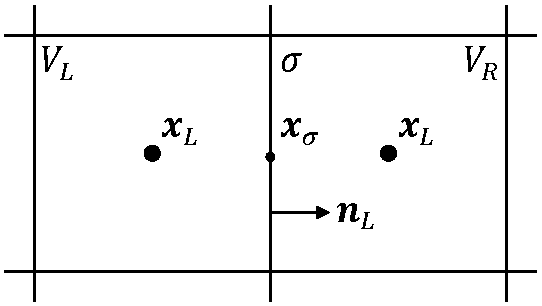
\includegraphics[width=0.6\textwidth]{cctpfa3.pdf}
	\caption[Two cells $V_L$ and $V_R$ sharing the face $\sigma$]{Two cells 
	$V_L$ and $V_R$ sharing the face $\sigma$.}
	\label{fig:cctpfa}
\end{figure}
Let us consider for instance the face $\sigma = \partial V_L \cup \partial 
V_R$, according to Figure~\ref{fig:cctpfa}, and let the permeability tensor be 
diagonal so that it act as a scalar. We approximate the derivative of the 
pressure $\partial p /\partial 
x$ with a centred finite difference:
\begin{equation}
\frac{\partial p}{\partial x} \approx \frac{p_R-p_L}{x_R -x_L}.
\end{equation}
We approximate the permeability $\mathbf{K}$ with its value at 
$\mathbf{x}_\sigma$, while 
for the viscosity $\mu$ (and eventually the density $\varrho$) we employ the 
upwind value.

In case of discontinuous permeabilities at the face $\sigma$, an harmonic 
average weighted on the distances between the cell centres and the face is 
performed:
\begin{equation}
\frac{|x_R - x_L|}{\mathrm{K}} \approx 
\frac{|x_\sigma - x_L|}{\mathrm{K}_L}+\frac{|x_R - x_\sigma|}{\mathrm{K}_R}.
\end{equation}

These formulas for the TPFA approximation are the simplified version for a 
Cartesian grid, while in the general case of an unstructured grid the method is 
derived exploiting a decomposition of the vector
\begin{equation}
\mathbf{d}_{L,\sigma}=\mathbf{x}_\sigma - \mathbf{x}_L,
\end{equation}
based the co-normal vector $\mathbf{Kn}_L$. Moreover it 
can be shown that this approximation is consistent only if the grid is 
K-orthogonal, i.e. if $\mathbf{Kn}_L$ is parallel to $\mathbf{d}_{L, \sigma}$ 
(see \cite{tesi:wolff}).
%\section{Coupling conditions}
% Disegno di cosa succede all'interfaccia
% Not sure about this section...
\section{Time discretization} \label{subsec:time}
For the temporal discretization we employ fully implicit, unconditionally 
stable methods as the Backward Euler (BE) and the Backward Differencing Formula 
2 (BDF2) also for non constant time steps. A monolithic approach is used, the 
Jacobian matrix is computed 
numerically then the UMFPACK solver is used. The time-step size depends of the 
convergence of the Newton's method at the previous time iteration.
\section{Summary}
Fully implicit coupling, monolithic approach, UMFPACK, cenni alle coupling 
conditions and boundary conditions, primary variables.